\documentclass{article}
\usepackage{graphicx}
\usepackage[utf8]{inputenc}
\usepackage[a4paper, total={6in, 8in}]{geometry}
\usepackage{fancyhdr}
\usepackage{subcaption}
\usepackage{float}
\usepackage[hidelinks]{hyperref}
\usepackage{xcolor}
\usepackage{enumitem}
\usepackage{graphicx}
\usepackage{tcolorbox}
\usepackage{array}

\pagestyle{fancy}
\fancyhf{}
\fancyfoot[L]{Alessandro Dori}
\fancyfoot[R]{\thepage}
\fancyhead[L]{Interazione Uomo Macchina}
\fancyhead[R]{SmartCycle}
\renewcommand{\headrulewidth}{0.4pt}
\renewcommand{\footrulewidth}{0.4pt}

\begin{document}
\begin{center}
    \Huge Progetto Interazione Uomo Macchina
        \vspace{0.5cm}

        \large A.A. 2024/2025 - Alessandro Dori 1843237
        \vspace{1cm}

        \large \textsf{\textbf{SmartCycle}}

        \includegraphics[width=0.3\textwidth, trim=110 110 110 110, clip]{img/SM.png}
\end{center}

\section{Storico Revisioni}
\begin{table}[H]
    \centering
    \renewcommand{\arraystretch}{1} % Aumenta lo spazio tra le righe per migliorare la leggibilità
    \begin{tabular}{|m{2cm}|m{3cm}|p{8cm}|}
        \hline
            \textbf{Revisione} & \textbf{Data} & \textbf{Modifiche} \\ \hline
            \centering 1 & \centering 06/12/2024 & \begin{tabular}[c]{@{}p{8cm}@{}}Inserimento sottotask (filtrare per Città) nello Storyboard del Task 1, correzione termine "post" con il termine "annuncio" nello Storyboard del Task 2, creazione Task 3\end{tabular} \\ \hline
            \centering 2 & \centering // & \begin{tabular}[c]{@{}p{8cm}@{}}//\end{tabular} \\ \hline
    \end{tabular}
    \label{tab:revisione}
\end{table}


\section{Obiettivo}
Il progetto nasce dall'idea di sviluppare un sistema digitale che aiuti a ridurre gli sprechi alimentari, ispirato al modello di Too Good To Go e Olio. 
L’idea principale è creare un sistema che permetta agli utenti di trovare e acquistare prodotti alimentari invenduti a prezzi ridotti, mettendoli in contatto con negozi, ristoranti, supermercati e vicini della loro zona.

L’obiettivo da un lato è di aiutare i commercianti a vendere cibi che altrimenti verrebbero sprecati e persone comuni a non sprecare cibo in procinto di scadenza, dall’altro offrire agli utenti un modo semplice per risparmiare e fare scelte sostenibili. 
Il sistema fornirà funzionalità come la ricerca per posizione, la prenotazione e il pagamento online, la possibilità di acquistare (in alcuni casi gratis) box di cibo invenduto o cibo in scadenza, e la visualizzazione di statistiche personali sull’impatto ambientale.

Questo sistema vuole risolvere un problema pratico, ma anche sensibilizzare le persone verso un consumo più consapevole e rispettoso dell’ambiente, contribuendo a ridurre l’impatto negativo dello spreco alimentare.

\section{Analisi delle App Simili}
\subsection{Too Good To Go}
L'applicazione Too Good To Go offre un servizio simile a quello che si vuole realizzare con SmartCycle.
Too Good To Go permette di acquistare cibo invenduto a prezzi ridotti, mettendo in contatto utenti e negozi della zona.
L'applicazione offre funzionalità come la ricerca dei locali per posizione, la possibilità di ordinare una box mista cibo invenduto e di prenotare e pagare direttamente dall'app.

\subsection{Olio}
Olio è un'applicazione che permette di acquistare cibo invenduto a prezzi ridotti, mettendo in contatto utenti e negozi della zona.
L'applicazione offre funzionalità come la possibilità di "scambiare" cibo invenduto con altri utenti, solitmente vicini demograficamente, il tutto gratuitamente.
Olio rappresenta un’evoluzione del concetto di economia circolare applicata al consumo domestico e alla sostenibilità.

\section{Needfinding}
Sono state condotte delle interviste per capire meglio le abitudini alimentari delle persone e le loro opinioni riguardo lo spreco alimentare, ma anche per capire quante persone al giorno d'oggi siano informate dell'esistenza di applicazioni come Too Good To Go e Olio.
In particolare sono state fatte domande riguardo la frequenza con cui si butta cibo, la frequenza con cui si ordina cibo a domicilio, la frequenza con cui si cucina, la frequenza con cui si fa la spesa, e la frequenza con cui si utilizzano applicazioni per acquistare cibo invenduto.

\subsection{Resoconto Interviste}
Dalle interviste svolte emerge un forte interesse per soluzioni mirate alla riduzione dello spreco alimentare. 
Gli intervistati si sono dimostrati molto consapevoli del problema e interessati all’idea di contribuire concretamente a contrastarlo.
\newline
L'idea è di creare un sistema che includa funzionalità che vadano a colmare le necessità emerse dalle interviste.

\subsection{Resoconto Questionario}
E' stato proposto un questionario per capire meglio quante persone siano informate dell'esistenza di applicazioni come Too Good To Go e Olio e le loro abitudini per quanto riguarda lo spreco alimentare.
\newline
Dai risultati del questionario emerge che:
\begin{itemize}
    \item La maggior parte delle persone intervistate non conosce applicazioni come Too Good To Go e Olio.
    \item Una buona parte delle persone intervistate butta cibo almeno una volta a settimana.
    \item Per la maggior parte delle persone è molto importante ridurre lo spreco alimentare.
    \item Molte persone sono disposte a spendere una fascia di prezzo tra i 5 e i 10 euro per acquistare cibo invenduto.
\end{itemize}
\newpage
\hbox{Seguono i risultati dettagliati delle principali risposte del questionario.}

\begin{figure}[H]
    \centering
    \begin{subfigure}{0.40\textwidth}
        \centering
        \includegraphics[width=\textwidth]{img/graphic.png}
        \caption{Utilizzo applicazioni per acquistare cibo invenduto}
    \end{subfigure}
    \hfill
    \begin{subfigure}{0.40\textwidth}
        \centering
        \includegraphics[width=\textwidth]{img/graphic2.png}
        \caption{Frequenza con cui si butta cibo}
    \end{subfigure}
\end{figure}

\begin{figure}[H]
    \centering
    \begin{subfigure}{0.40\textwidth}
        \centering
        \includegraphics[width=\textwidth]{img/graphic3.png}
        \caption{Importanza riduzione spreco alimentare}
    \end{subfigure}
    \hfill
    \begin{subfigure}{0.40\textwidth}
        \centering
        \includegraphics[width=\textwidth]{img/graphic4.png}
        \caption{Fascia di prezzo per acquistare cibo invenduto}
    \end{subfigure}
\end{figure}

\hbox{A seguito delle interviste e dei questionari sono emersi i seguenti \textbf{Need}:}
\begin{enumerate}[label=\textbf{Need-\arabic*}]
    \item Possibilità di pagare una box di cibo invenduto per donarla a chi ne ha bisogno. \label{need1}
    \item Gli utenti sono interessati a non sprecare cibo e a ridurre lo spreco alimentare. \label{need2}
    \item Necessità di fasce orarie di ritiro del cibo invenduto più flessibili (inserire la fascia oraria come parametro di ricerca). \label{need3}
    \item Sapere prima dell'acquisto la quantità di cibo della box (per esempio, quanti pasti si possono preparare/coprire con il cibo ricevuto). \label{need4}
    \item Ricevere una possibile ricetta consigliata per il cibo ricevuto, così da poterlo utilizzare al meglio (nel caso in cui il contenuto della box sia da preparare). \label{need5}
    \item Gli utenti necessitano di un servizio di consegna a domicilio del cibo invenduto (solo in bici o con mezzi elettrici per coerenza con l'ecosostenibilità) \label{need6}
    \item Possibilità di filtrare i risultati dei locali. \label{need7}
    \item Possibilità di pagamento online. \label{need8}
\end{enumerate}



\newpage
\subsection{Task Analysis}
A seguito delle interviste e dei risultati del questionario, sono stati identificati i task principali che l'utente potrà svolgere con SmartCycle.
\newline
I \textbf{task} principali sono:
\begin{enumerate}[label=\textbf{Task-\arabic*}]
    \item L'utente filtra i risultati dei locali per disponibilità di donazione a persone bisognose e Città, sceglie un locale e acquista una delle box predefinite di cibo invenduto da donare.
    \begin{itemize}
        \item Risolve il \hyperref[need1]{\textcolor{blue}{Need 1}} e \hyperref[need7]{\textcolor{blue}{Need 7}}.
        \item \textbf{Sottotask:} 
        \begin{itemize}
            \item Filtrare i risultati dei locali per disponibilità di donazione e Città.
            \item Scegliere un locale da cui acquistare una box di cibo invenduto da donare e scegliere anche una delle box predefinite disponibili (box standard, non personalizzabili).
            \item Acquistare una box di cibo invenduto da donare.
        \end{itemize}
    \end{itemize}
    \item L'utente annuncia la disponibilità di cibo invenduto da regalare/vendere, fornendo informazioni/foto sul cibo e la quantità disponibile.
    \begin{itemize}
        \item Risolve il \hyperref[need2]{\textcolor{blue}{Need 2}}.
        \item \textbf{Sottotask:} 
        \begin{itemize}
            \item Inserire informazioni sul cibo da regalare/vendere.
            \item Inserire la quantità disponibile del cibo.
            \item Inserire una foto del cibo disponibile.
        \end{itemize}
    \end{itemize}
    \item L'utente filtra i risultati dei locali per Città e fascia oraria di ritiro/consegna del cibo invenduto, sceglie un locale e acquista una box di cibo invenduto con consegna.
    \begin{itemize}
        \item Risolve il \hyperref[need3]{\textcolor{blue}{Need 3}}, \hyperref[need7]{\textcolor{blue}{Need 7}} e \hyperref[need8]{\textcolor{blue}{Need 8}}.
        \item \textbf{Sottotask:} 
        \begin{itemize}
            \item Filtrare i risultati dei locali per fascia oraria e Città e disponibilità di consegna.
            \item Scegliere un locale da cui acquistare una box di cibo invenduto.
            \item Acquista una box di cibo invenduto con consegna.
        \end{itemize}
    \end{itemize}
    \item L'utente dopo aver scelto il locale, visualizza la quantità di cibo della box (porzioni) ed eventualmente riceve una ricetta consigliata per il cibo acquistato (nel caso in cui la box contenga cibo da preparare).
    \begin{itemize}
        \item Risolve il \hyperref[need4]{\textcolor{blue}{Need 4}} e \hyperref[need5]{\textcolor{blue}{Need 5}}.
        \item \textbf{Sottotask:} 
        \begin{itemize}
            \item Visualizzare la quantità di cibo della box (porzioni).
            \item Ricevere una ricetta consigliata per il cibo acquistato.
        \end{itemize}
    \end{itemize}
    \item L'utente sceglie un locale, acquista una box di cibo invenduto e dopo aver comunicato il proprio indirizzo richiede la consegna a domicilio.
    \begin{itemize}
        \item Risolve il \hyperref[need6]{\textcolor{blue}{Need 6}}.
        \item \textbf{Sottotask:} 
        \begin{itemize}
            \item Scegliere un locale.
            \item Acquistare una box di cibo invenduto.
            \item Comunicare l'indirizzo per la consegna a domicilio.
            \item Richiedere la consegna a domicilio.
        \end{itemize}
    \end{itemize}
    \item L'utente filtra i risultati dei locali per disponibilità di pagamento online, sceglie un locale e acquista una box di cibo invenduto.
    \begin{itemize}
        \item Risolve il \hyperref[need8]{\textcolor{blue}{Need 8}} e \hyperref[need7]{\textcolor{blue}{Need 7}}.
        \item \textbf{Sottotask:} 
        \begin{itemize}
            \item Filtrare i risultati dei locali per disponibilità di pagamento online.
            \item Scegliere un locale da cui acquistare una box di cibo invenduto.
            \item Acquistare una box di cibo invenduto con pagamento online.
        \end{itemize}
    \end{itemize}
\end{enumerate}
    

\section{Storyboard}

\subsection{Task 1}
L'utente filtra i risultati dei locali per disponibilità di donazione a persone bisognose e Città, sceglie un locale e acquista una delle box predefinite di cibo invenduto da donare.
\begin{figure}[H]
    \centering
    \begin{tabular}{ccc}
        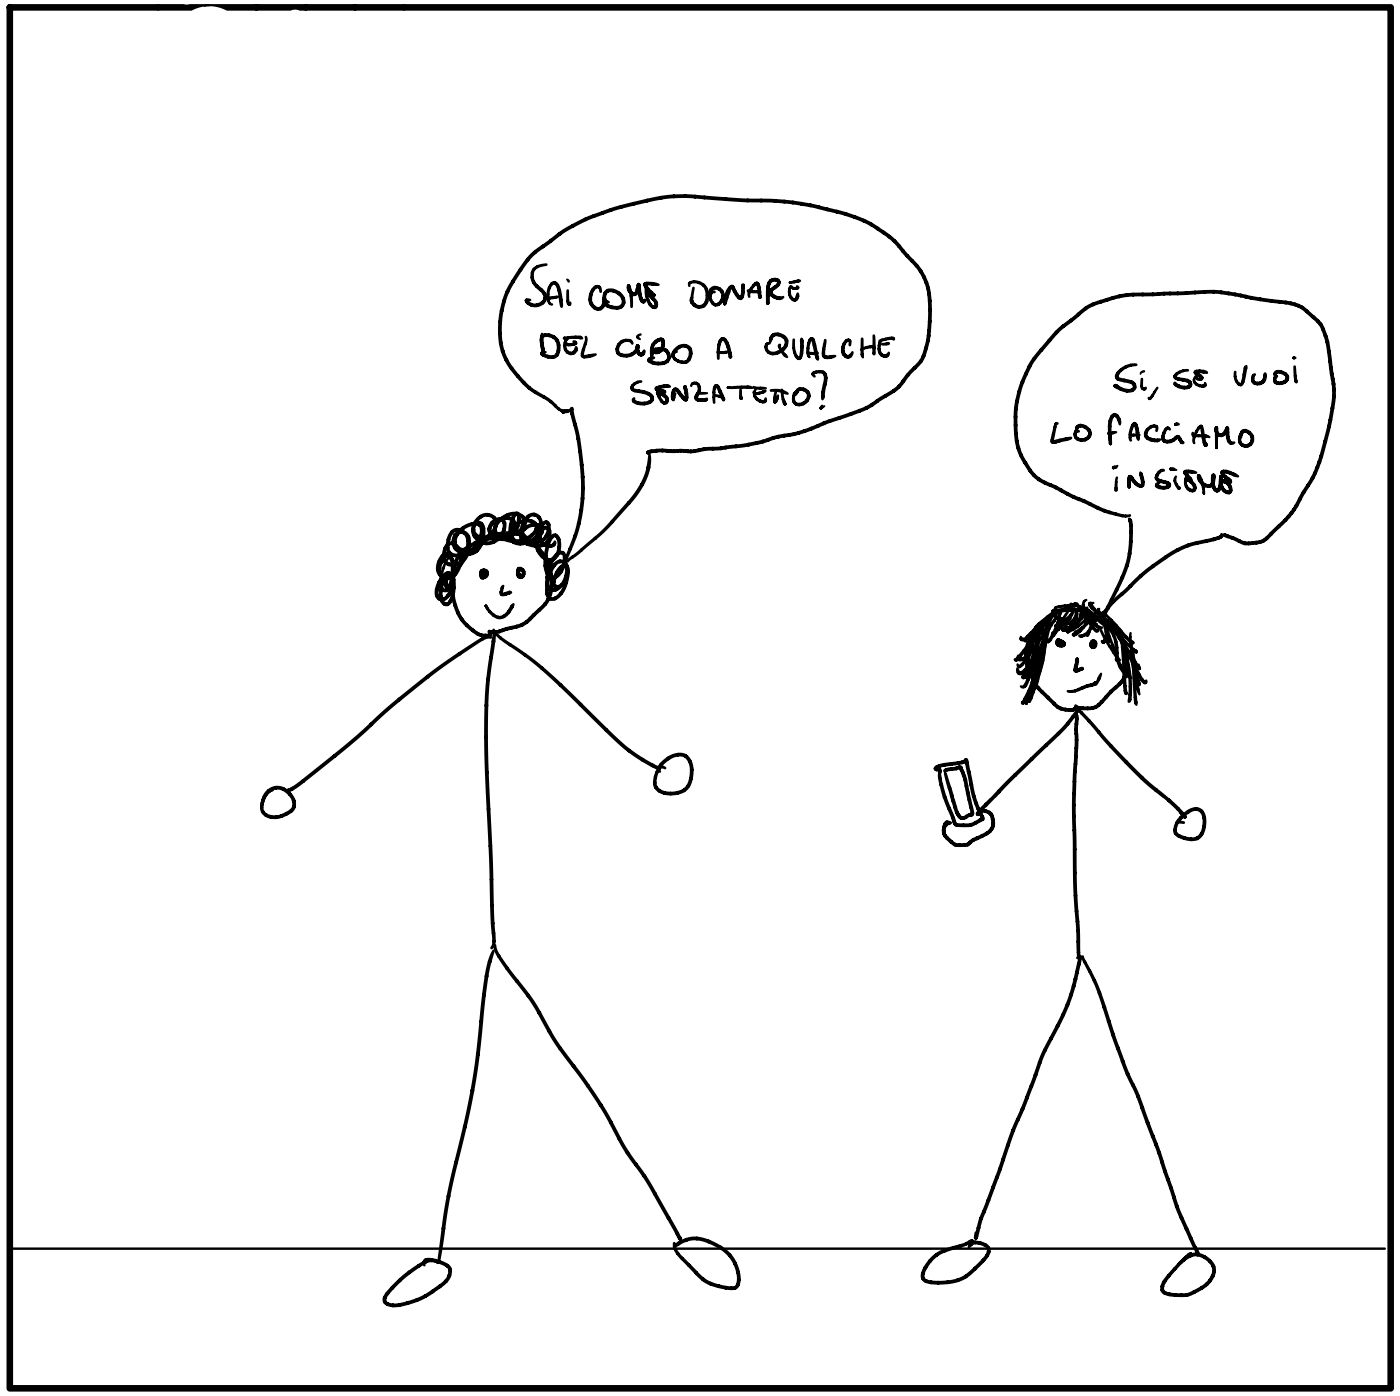
\includegraphics[width=0.3\textwidth]{Storyboard/task1-img II versione/t1.1.png} &
        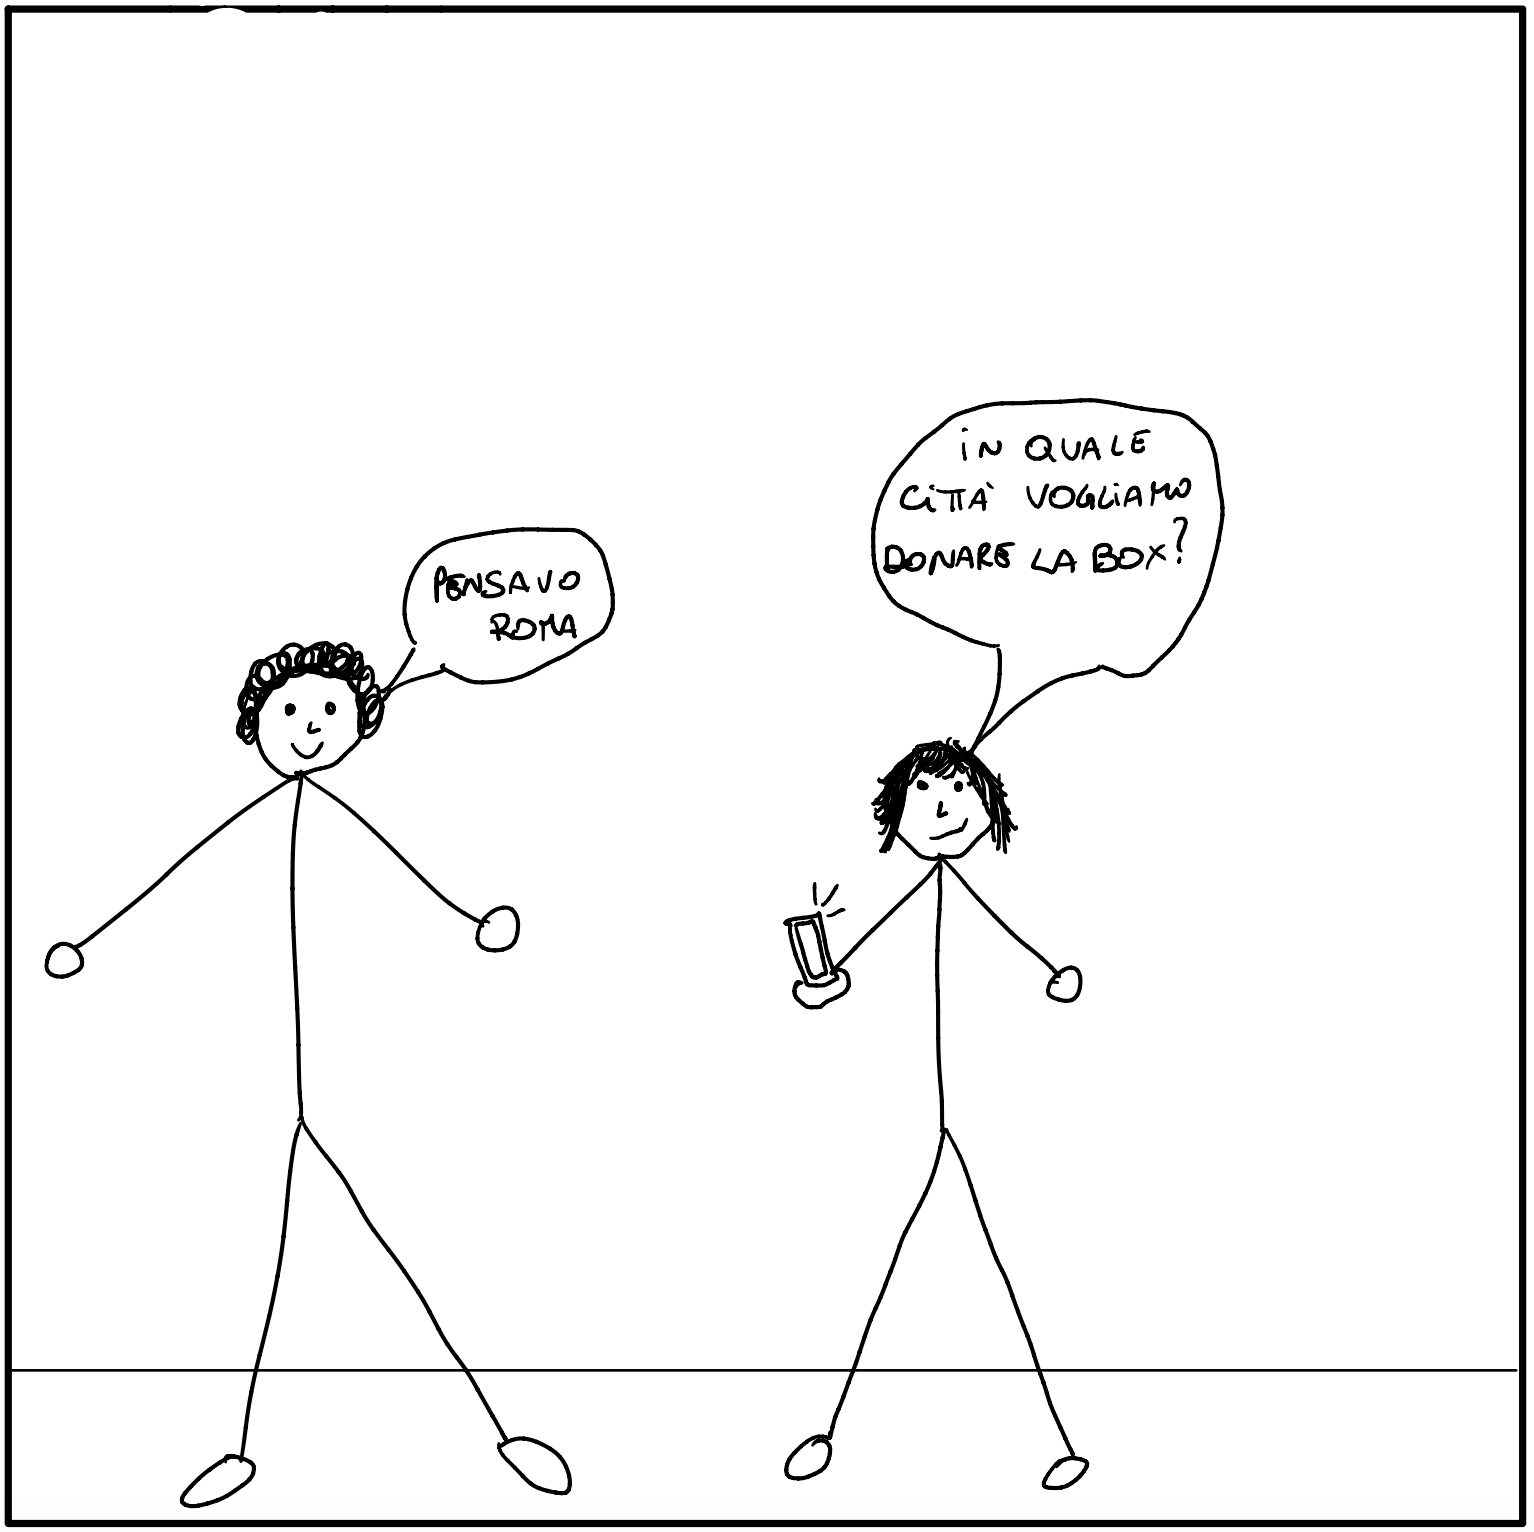
\includegraphics[width=0.3\textwidth]{Storyboard/task1-img II versione/t1.2.png} &
        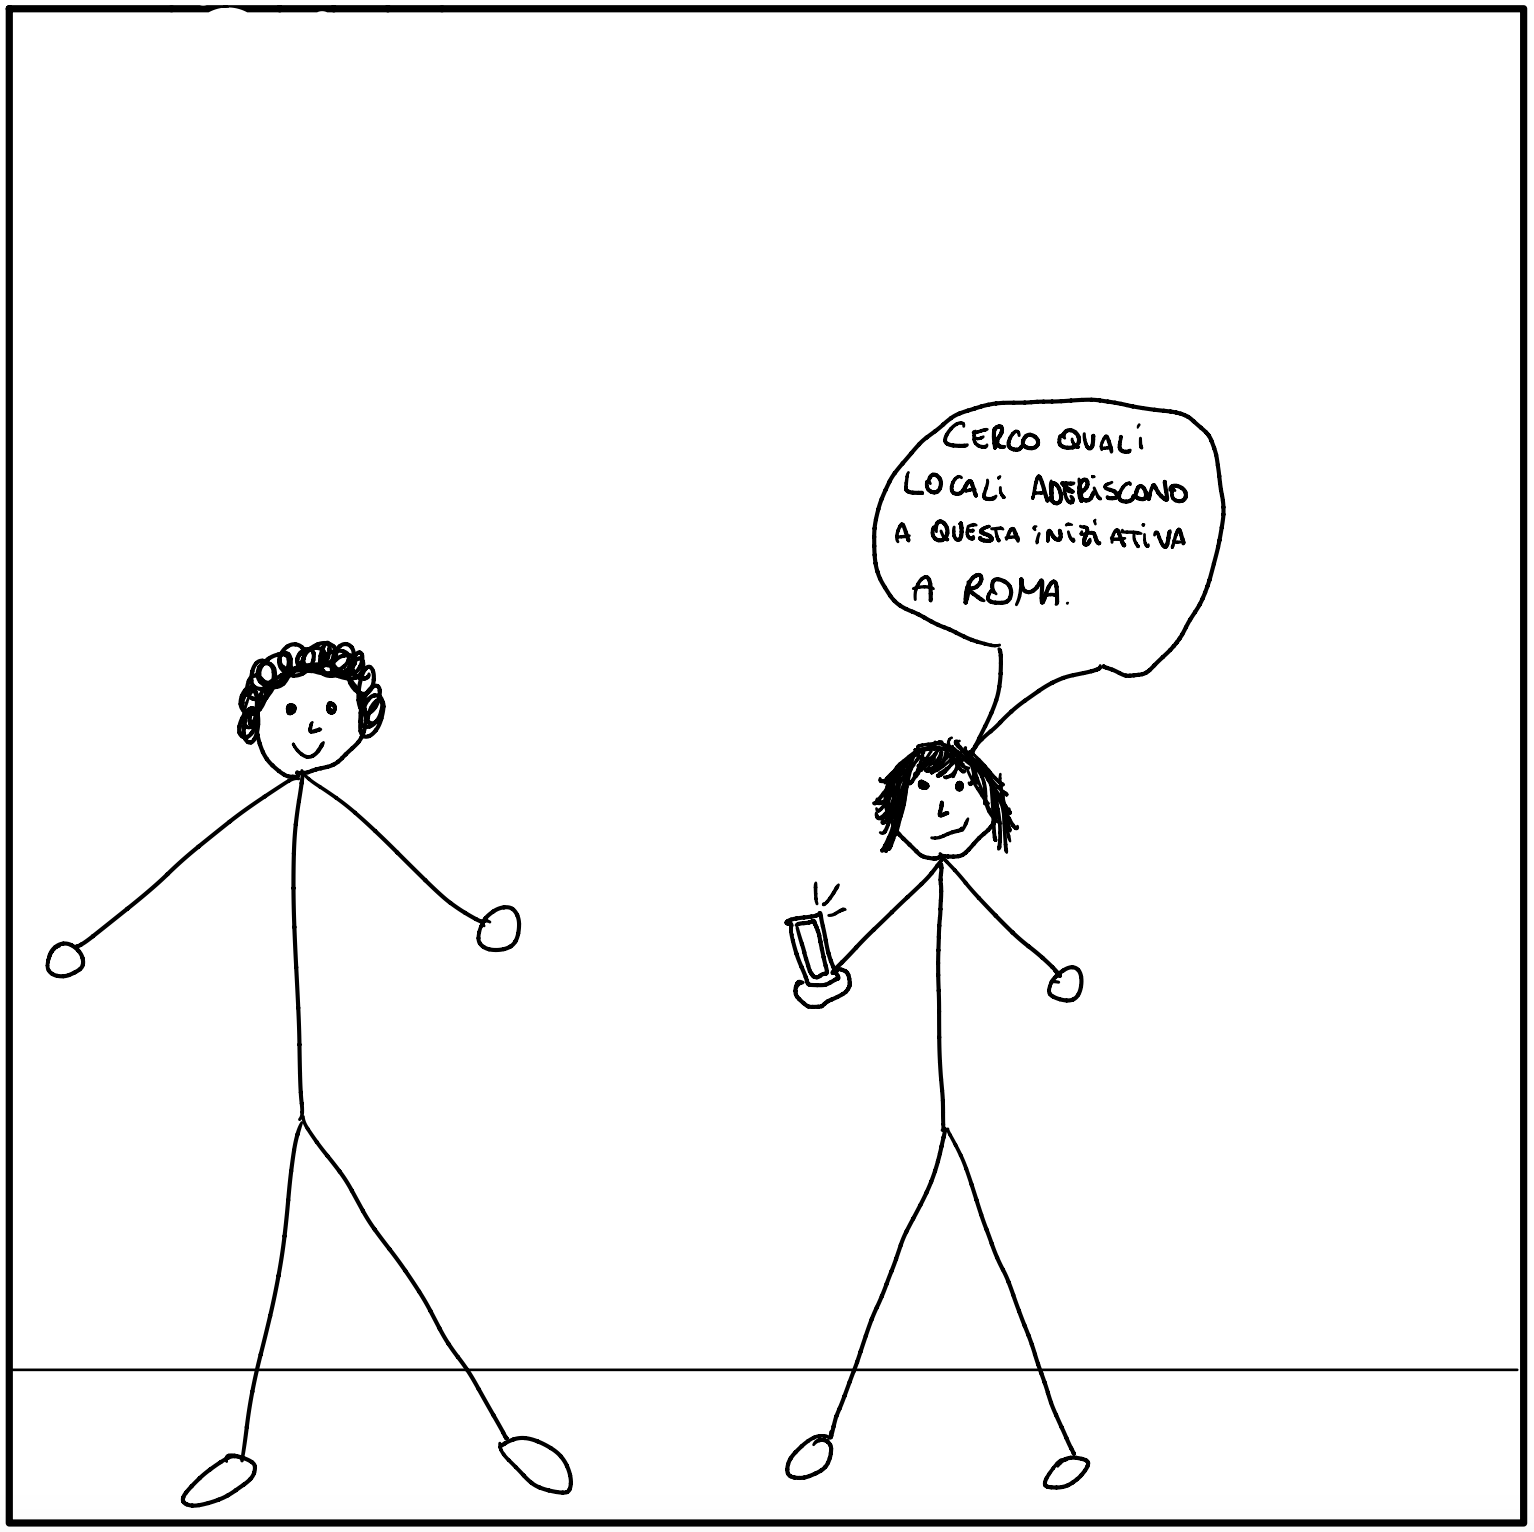
\includegraphics[width=0.3\textwidth]{Storyboard/task1-img II versione/t1.3.png} \\
        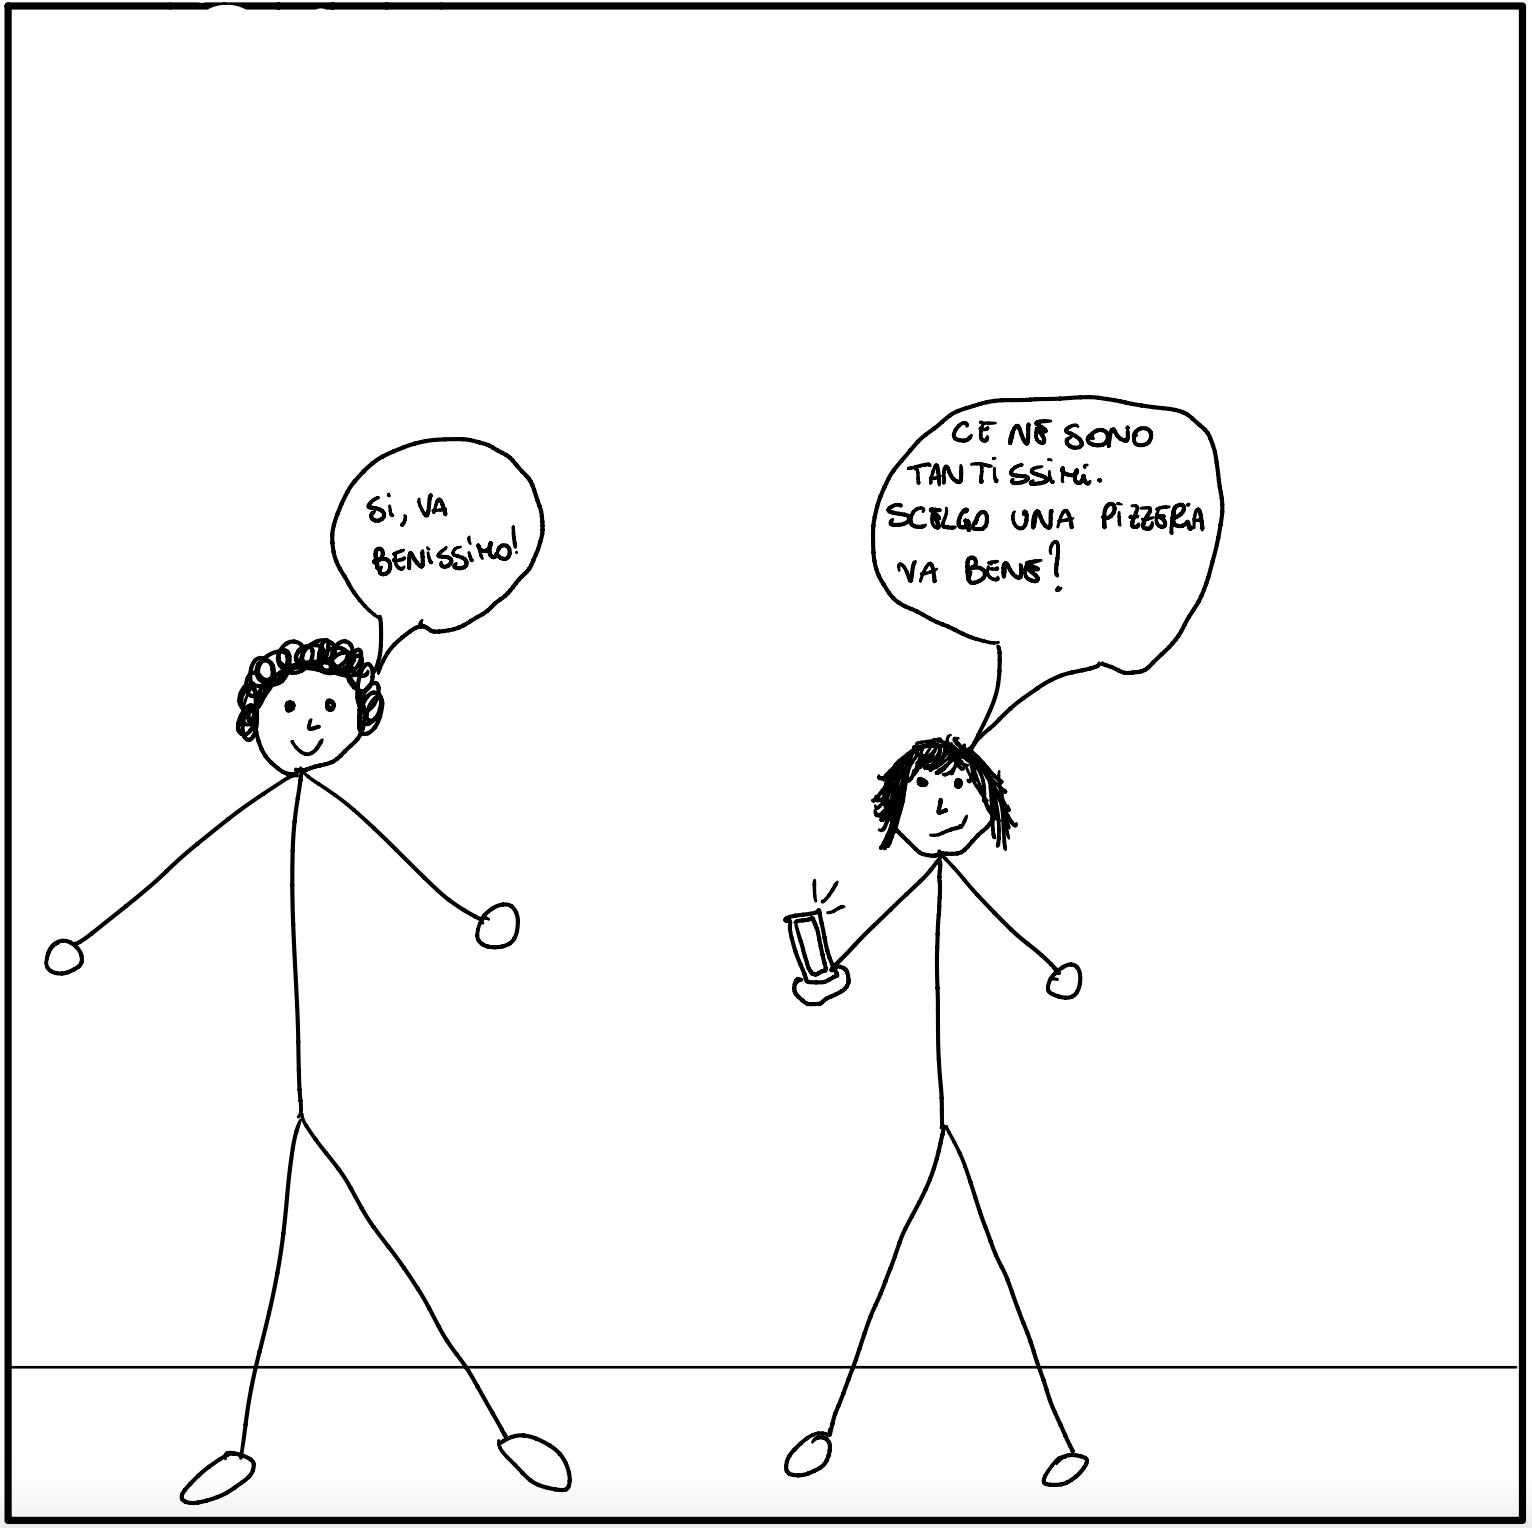
\includegraphics[width=0.3\textwidth]{Storyboard/task1-img II versione/t1.4.png} &
        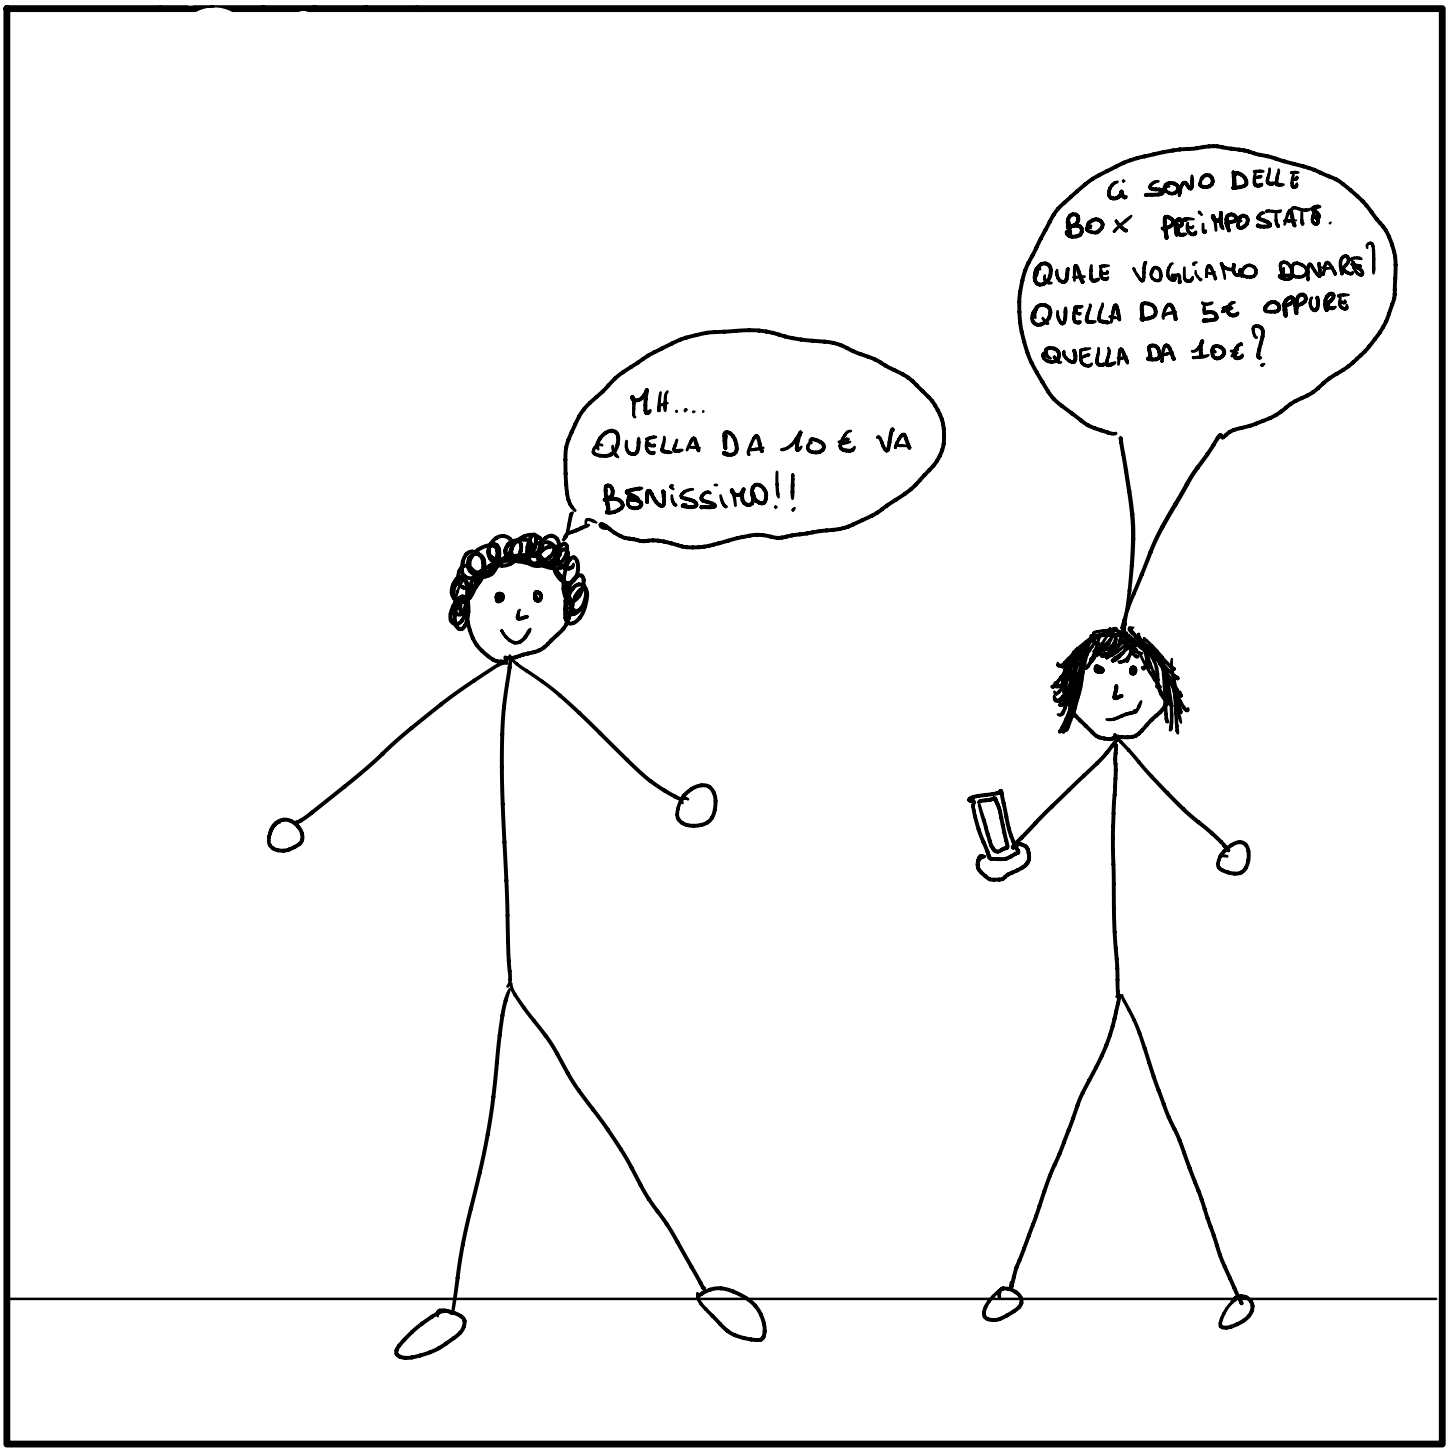
\includegraphics[width=0.3\textwidth]{Storyboard/task1-img II versione/t1.5.png} &
        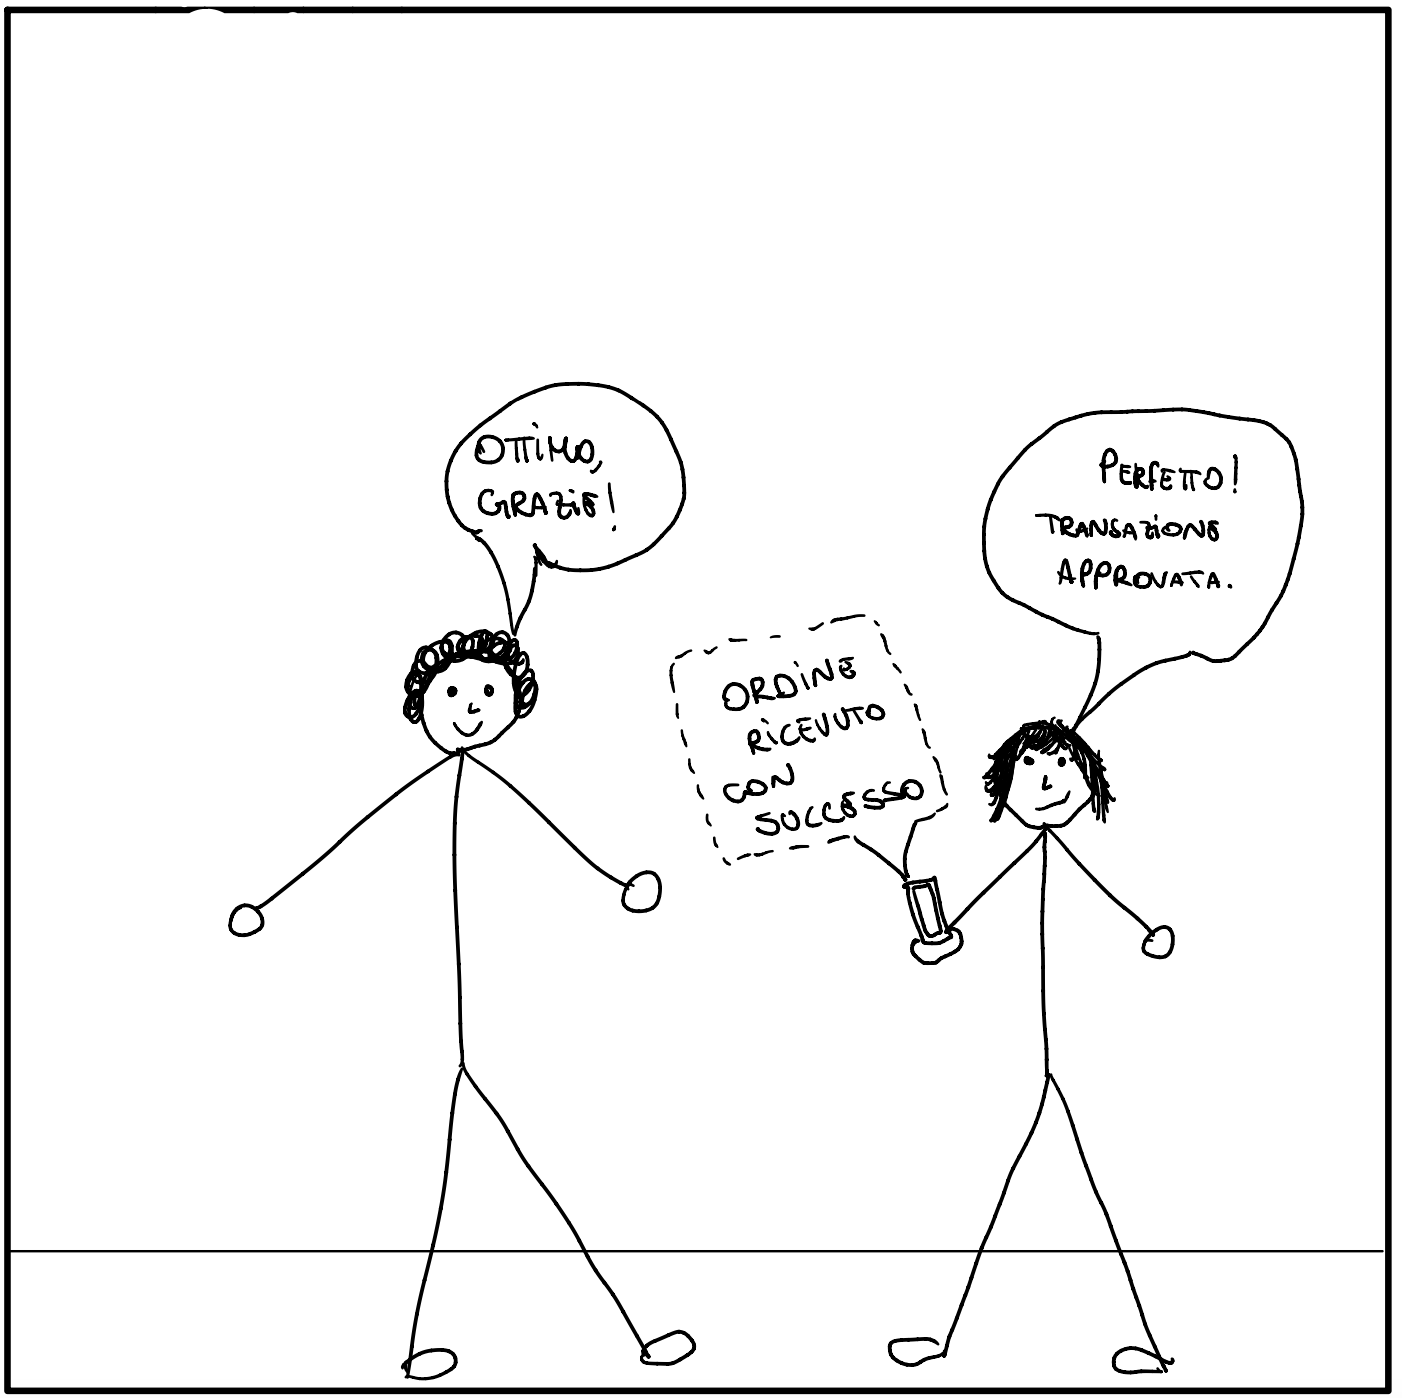
\includegraphics[width=0.3\textwidth]{Storyboard/task1-img II versione/t1.6.png} \\
    \end{tabular}
    \label{fig:task1}
\end{figure}


\newpage
\subsection{Task 2}
L'utente annuncia la disponibilità di cibo invenduto da regalare/vendere, fornendo informazioni/foto sul cibo e la quantità disponibile.
\begin{figure}[H]
    \centering
    \begin{tabular}{ccc}
        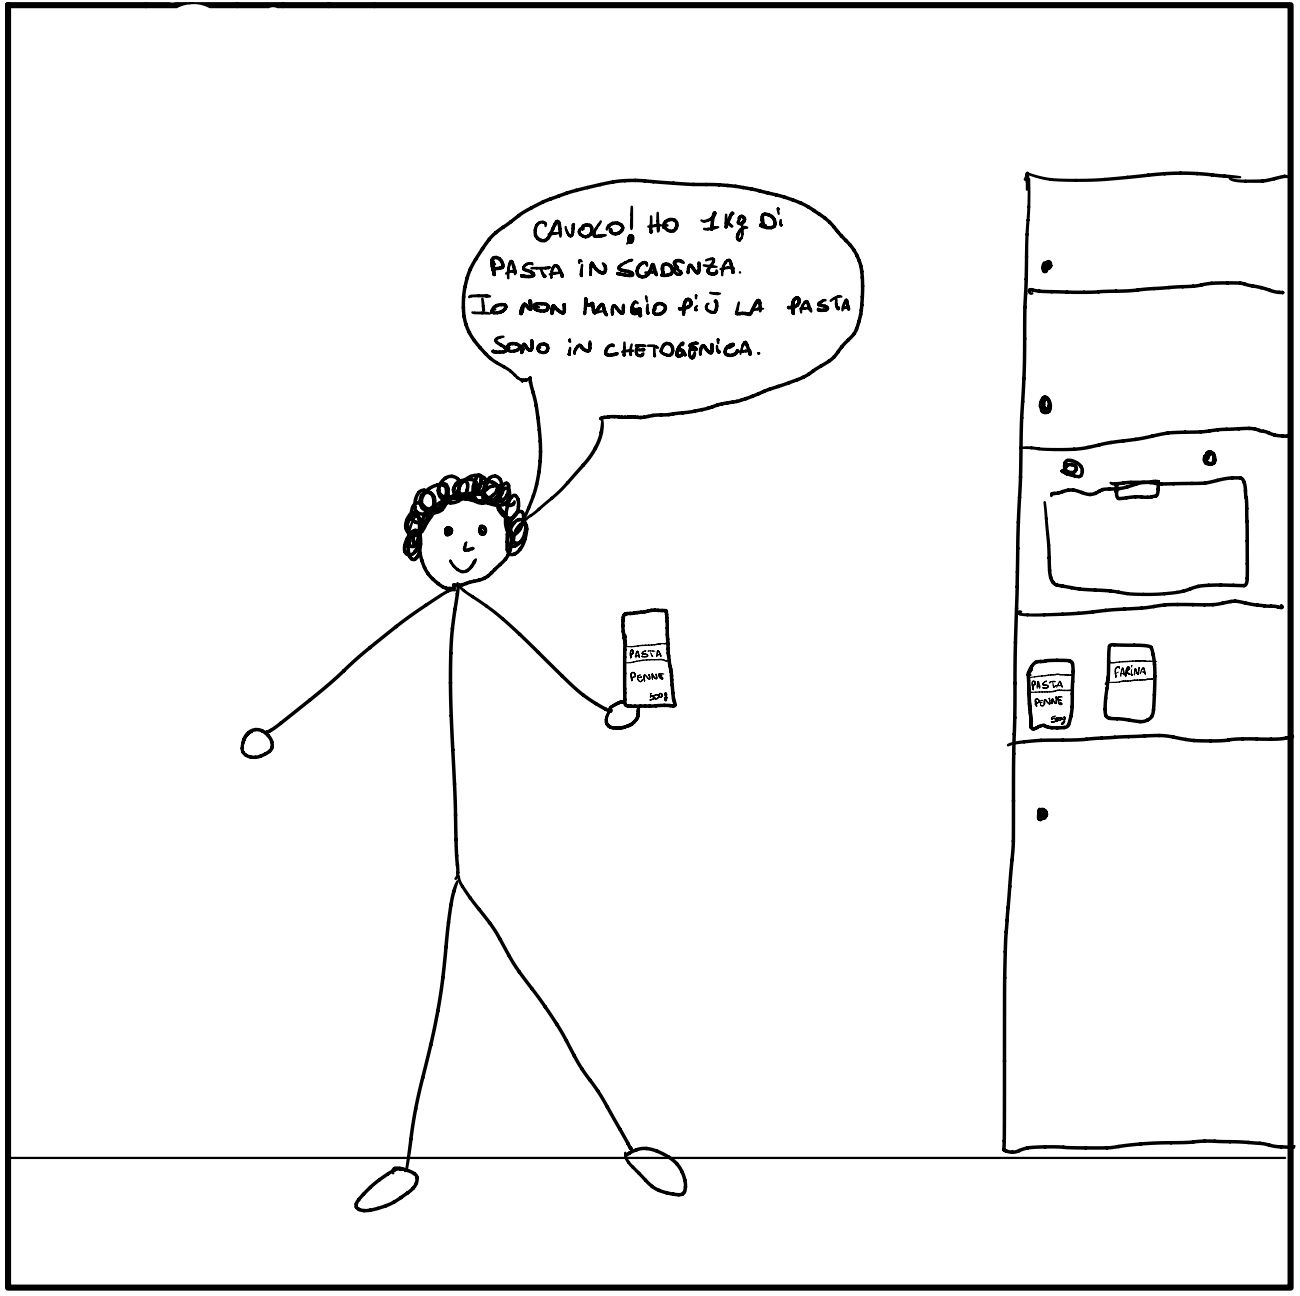
\includegraphics[width=0.3\textwidth]{Storyboard/task2-img II versione/t2.1.png} &
        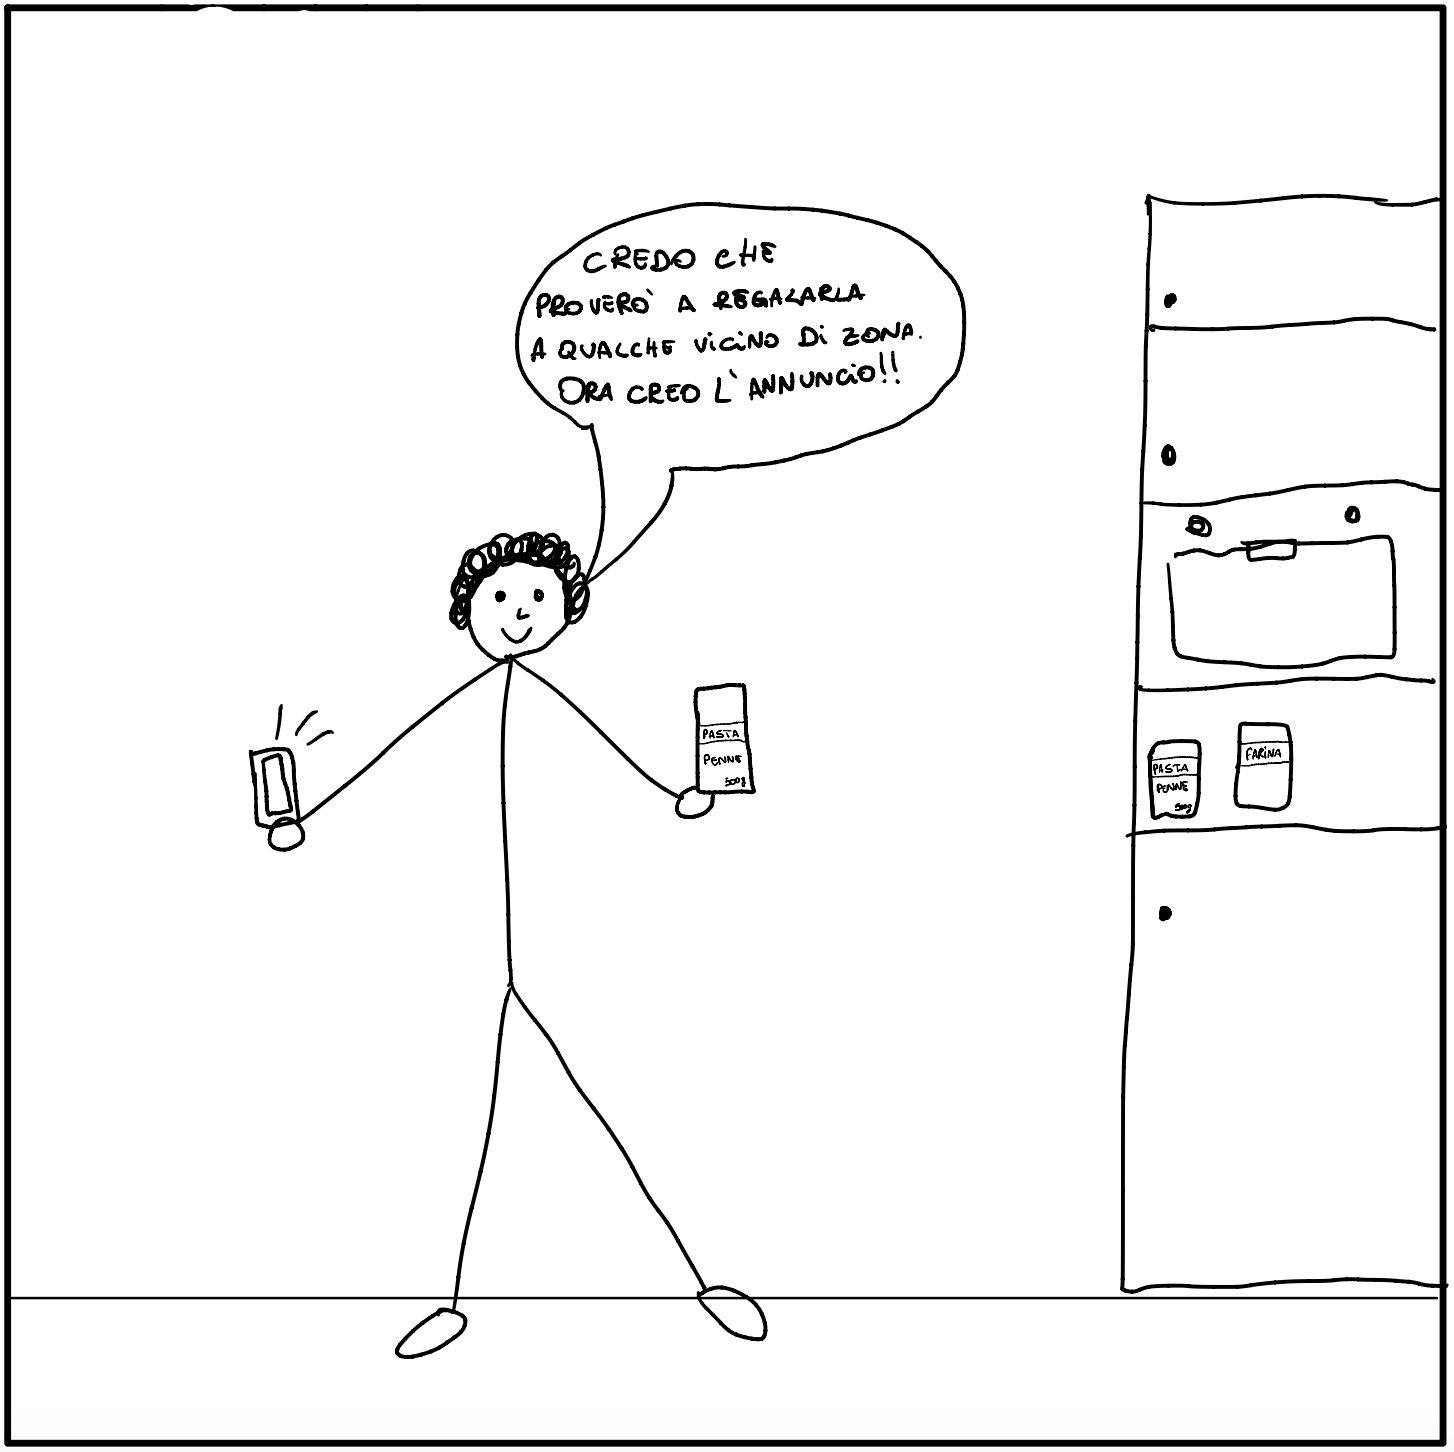
\includegraphics[width=0.3\textwidth]{Storyboard/task2-img II versione/t2.2.png} &
        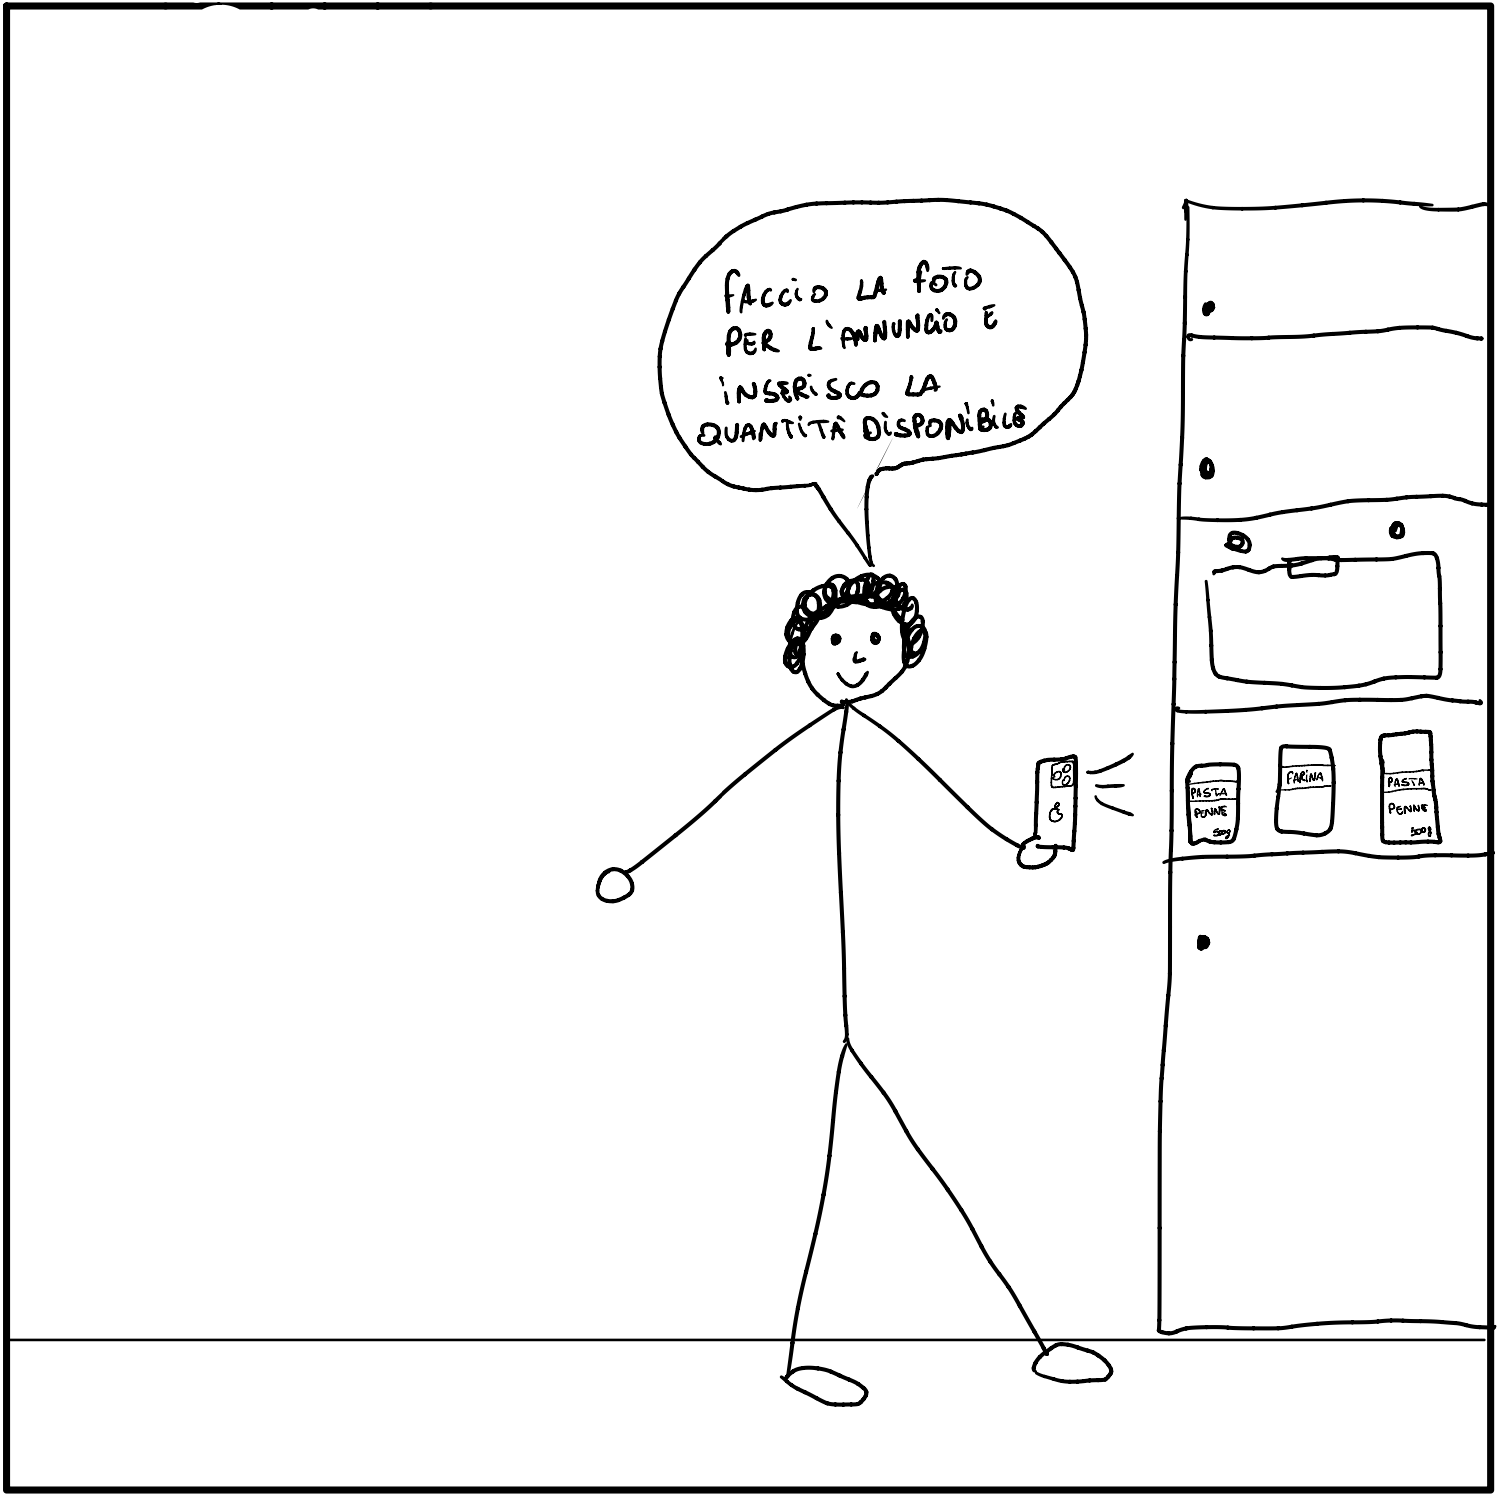
\includegraphics[width=0.3\textwidth]{Storyboard/task2-img II versione/t2.3.png} \\
        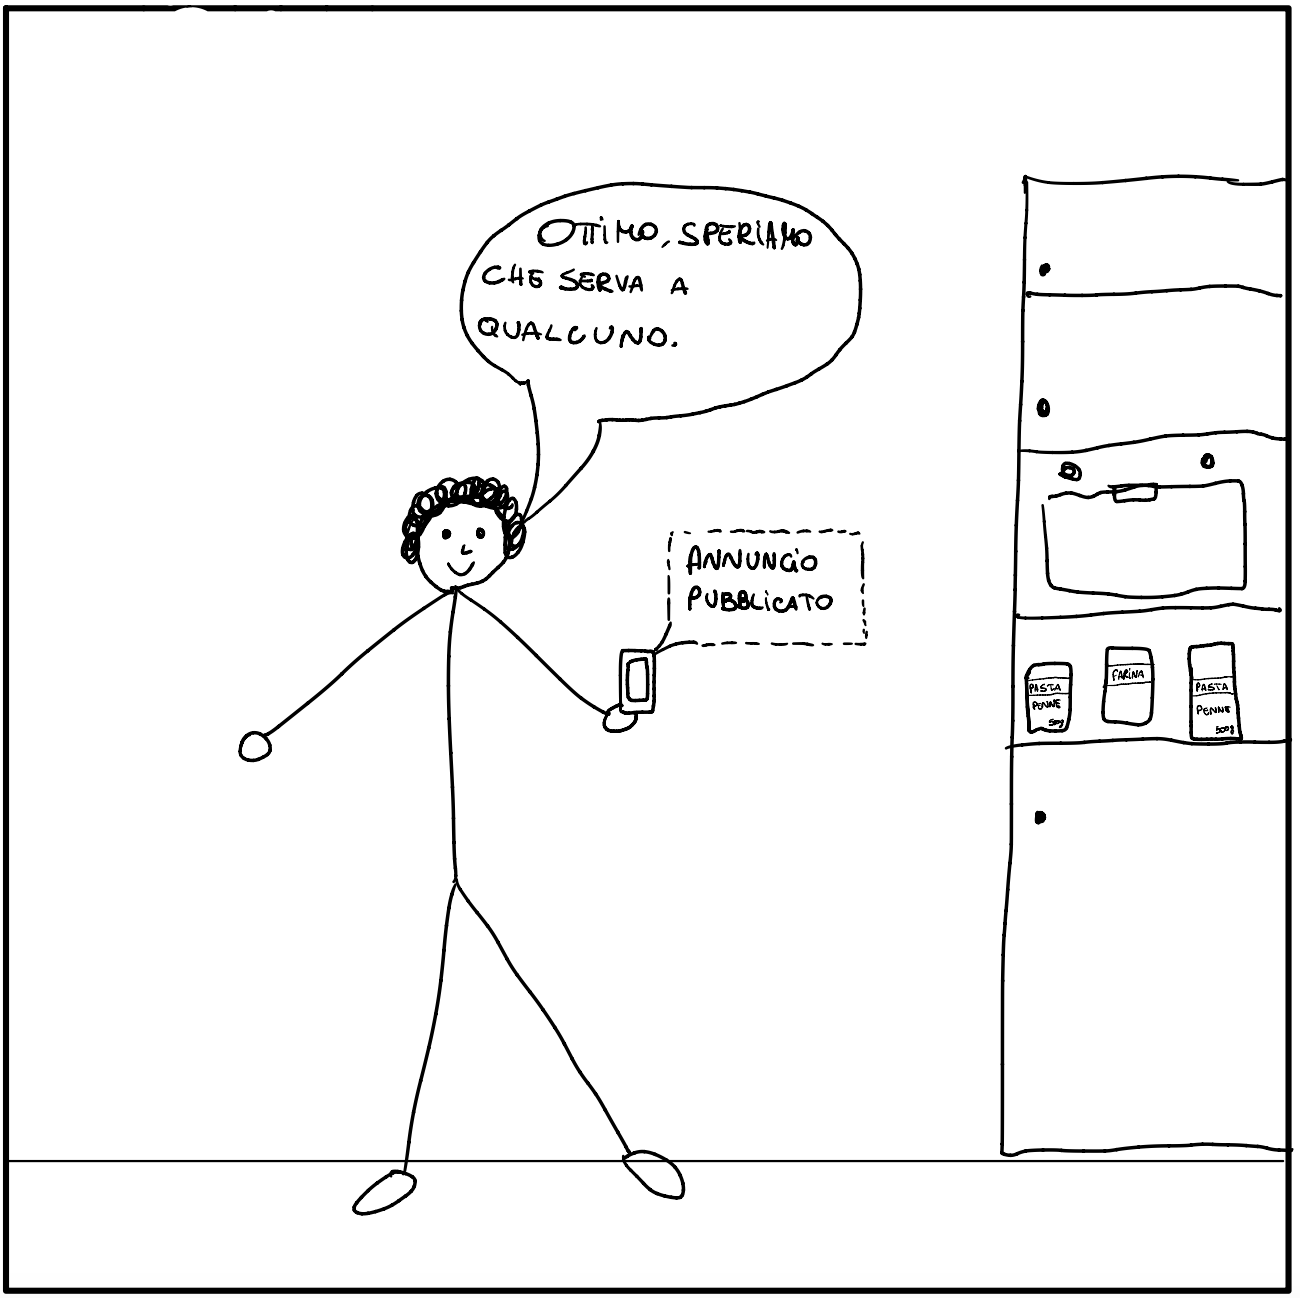
\includegraphics[width=0.3\textwidth]{Storyboard/task2-img II versione/t2.4.png} & & \\
    \end{tabular}
    \label{fig:task2}
\end{figure}

\newpage
\subsection{Task 3}
L'utente filtra i risultati dei locali per Città e fascia oraria di ritiro/consegna del cibo invenduto, sceglie un locale e acquista una box di cibo invenduto con consegna.
\begin{figure}[H]
    \centering
    \begin{tabular}{ccc}
        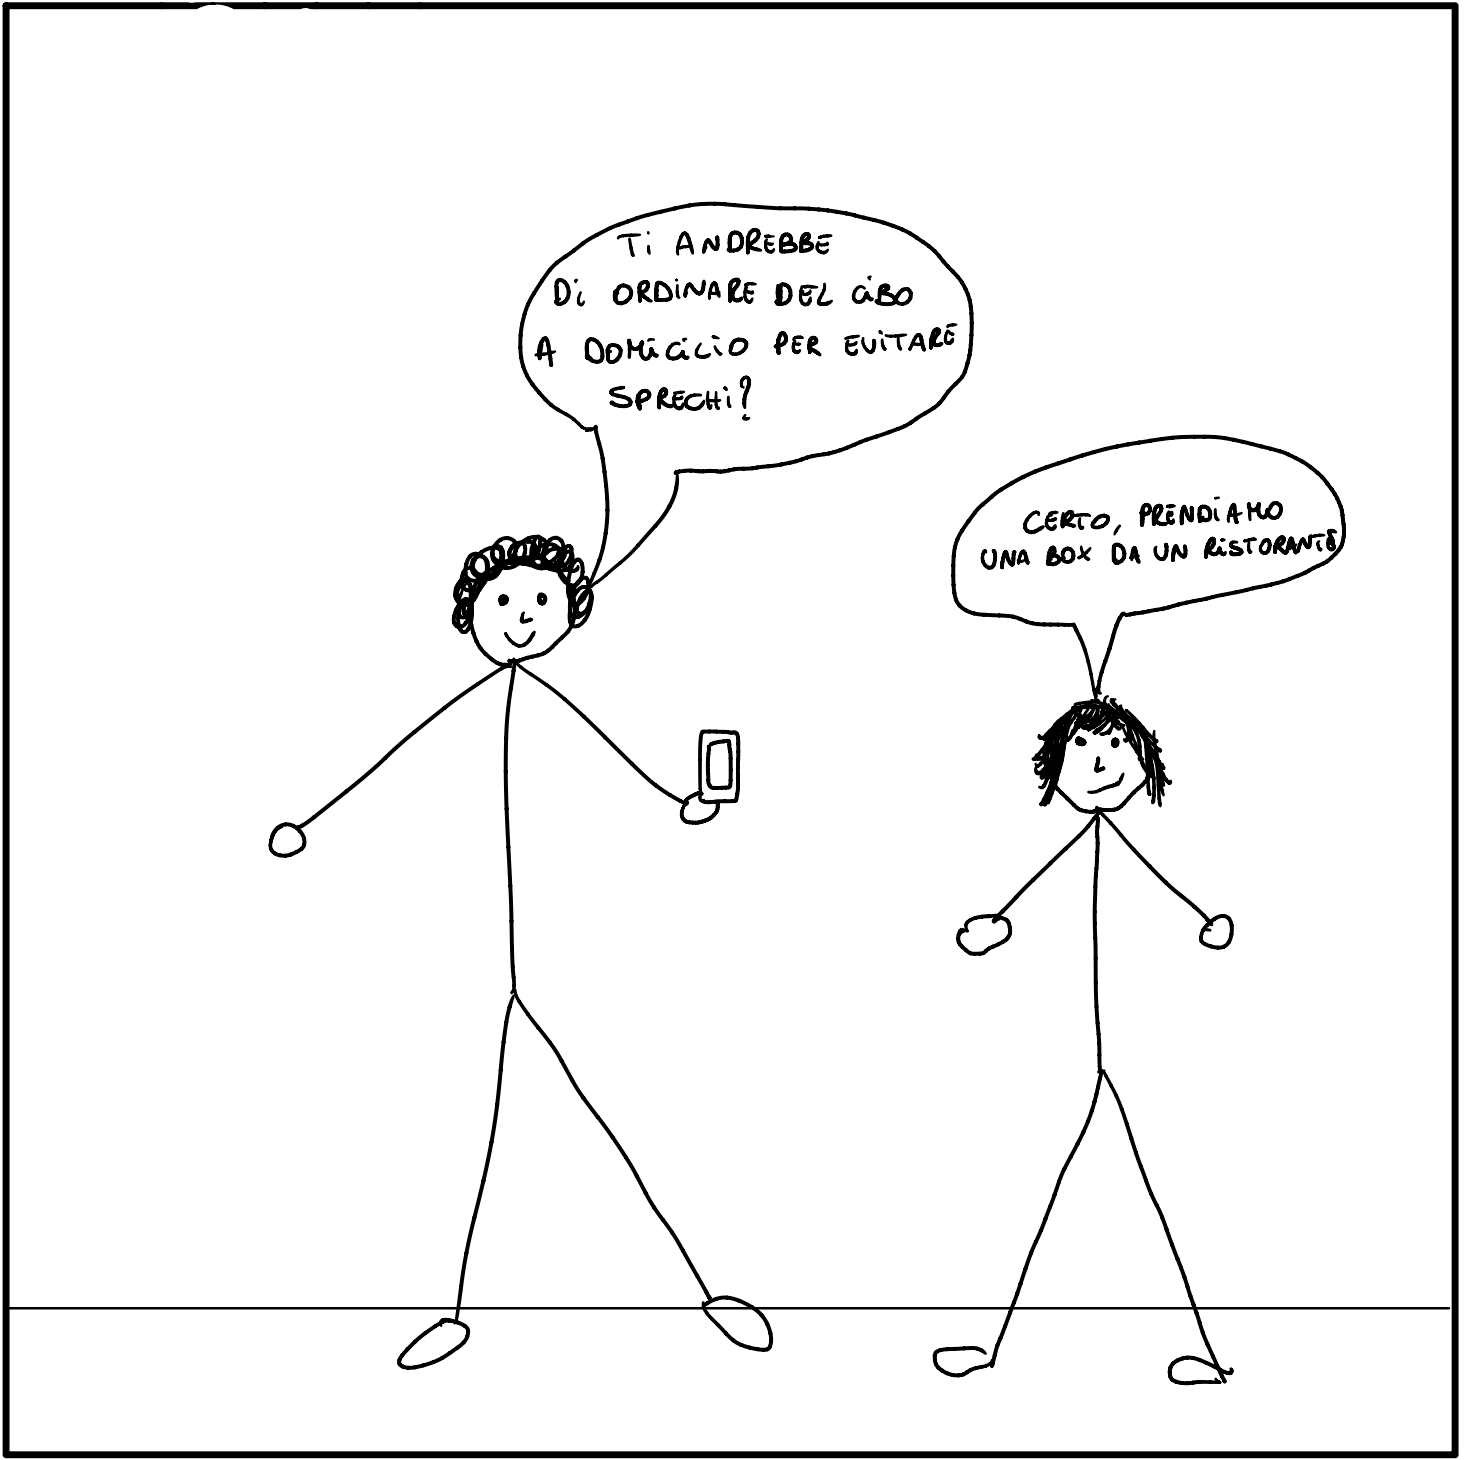
\includegraphics[width=0.3\textwidth]{Storyboard/task3-img/t3.1.png} &
        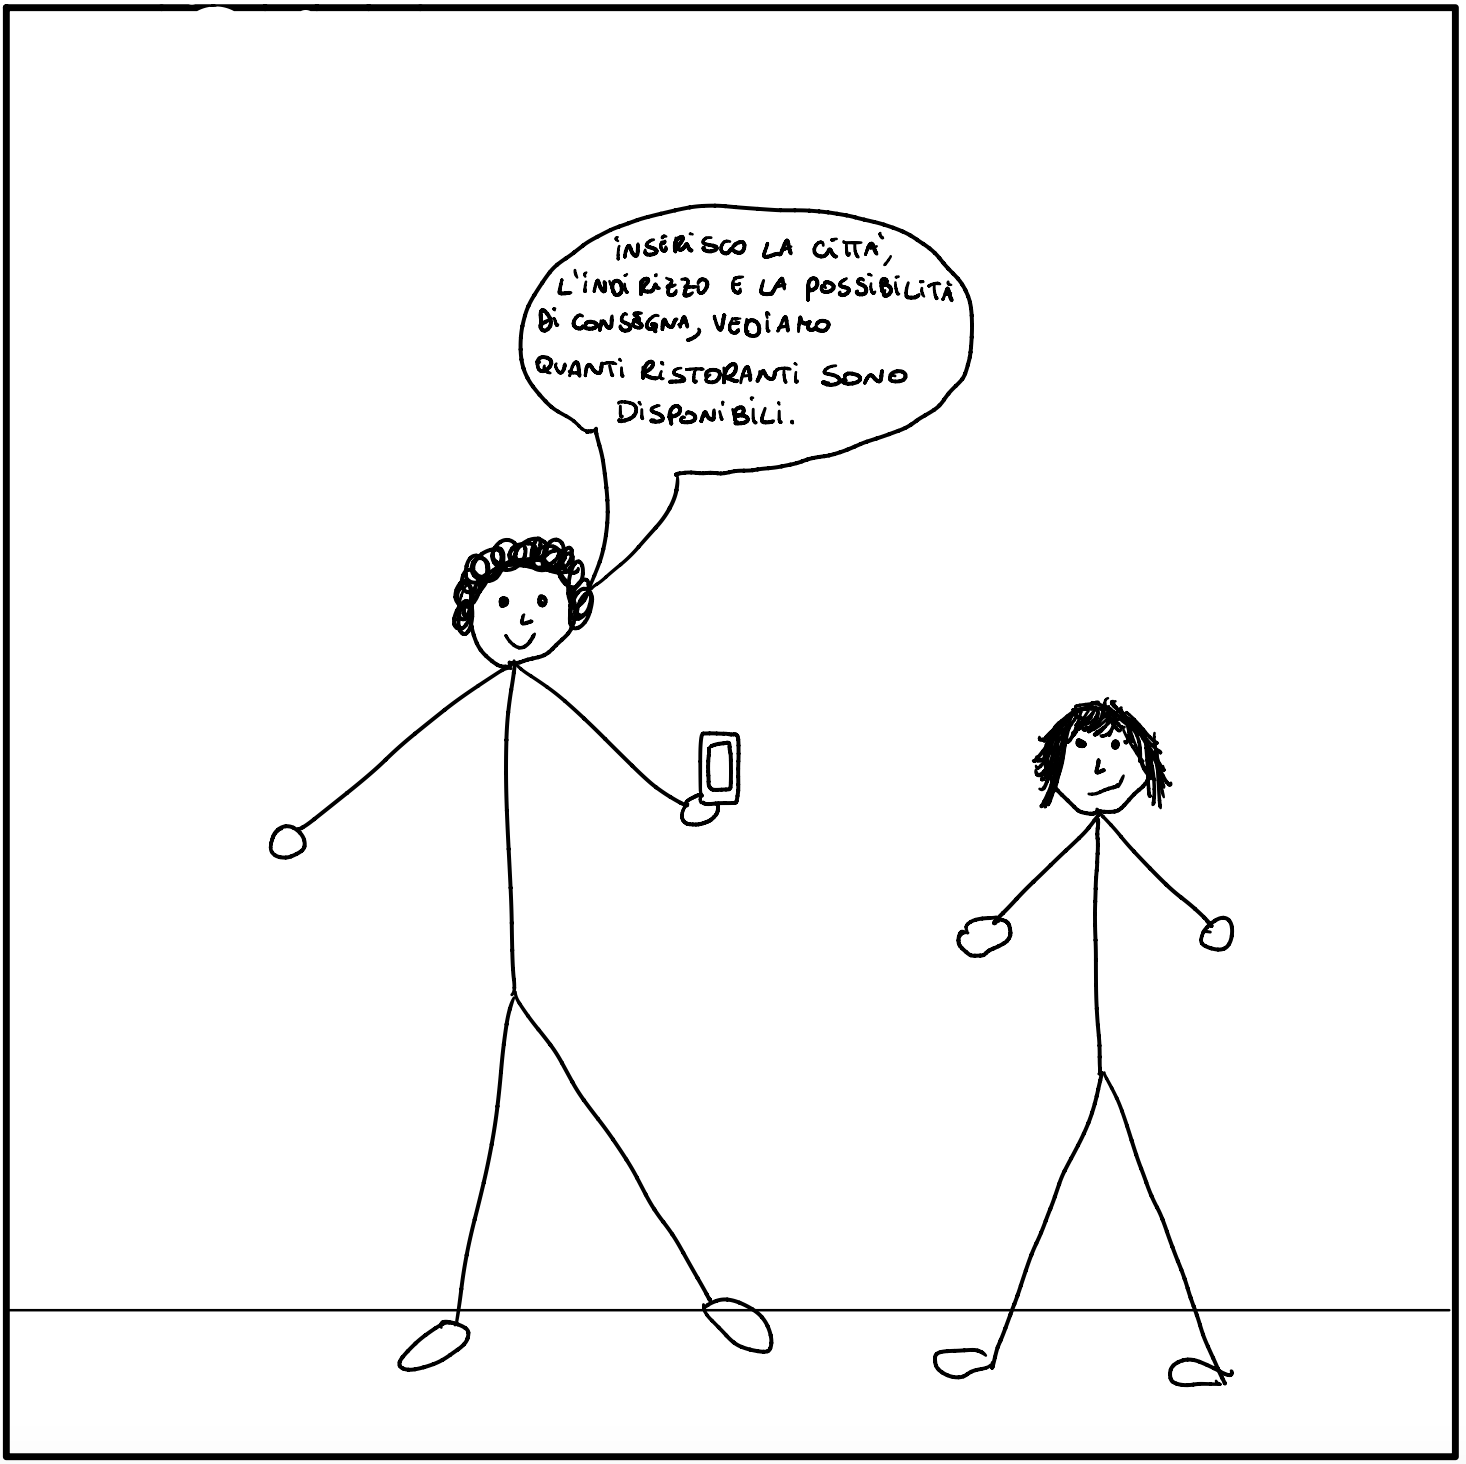
\includegraphics[width=0.3\textwidth]{Storyboard/task3-img/t3.2.png} &
        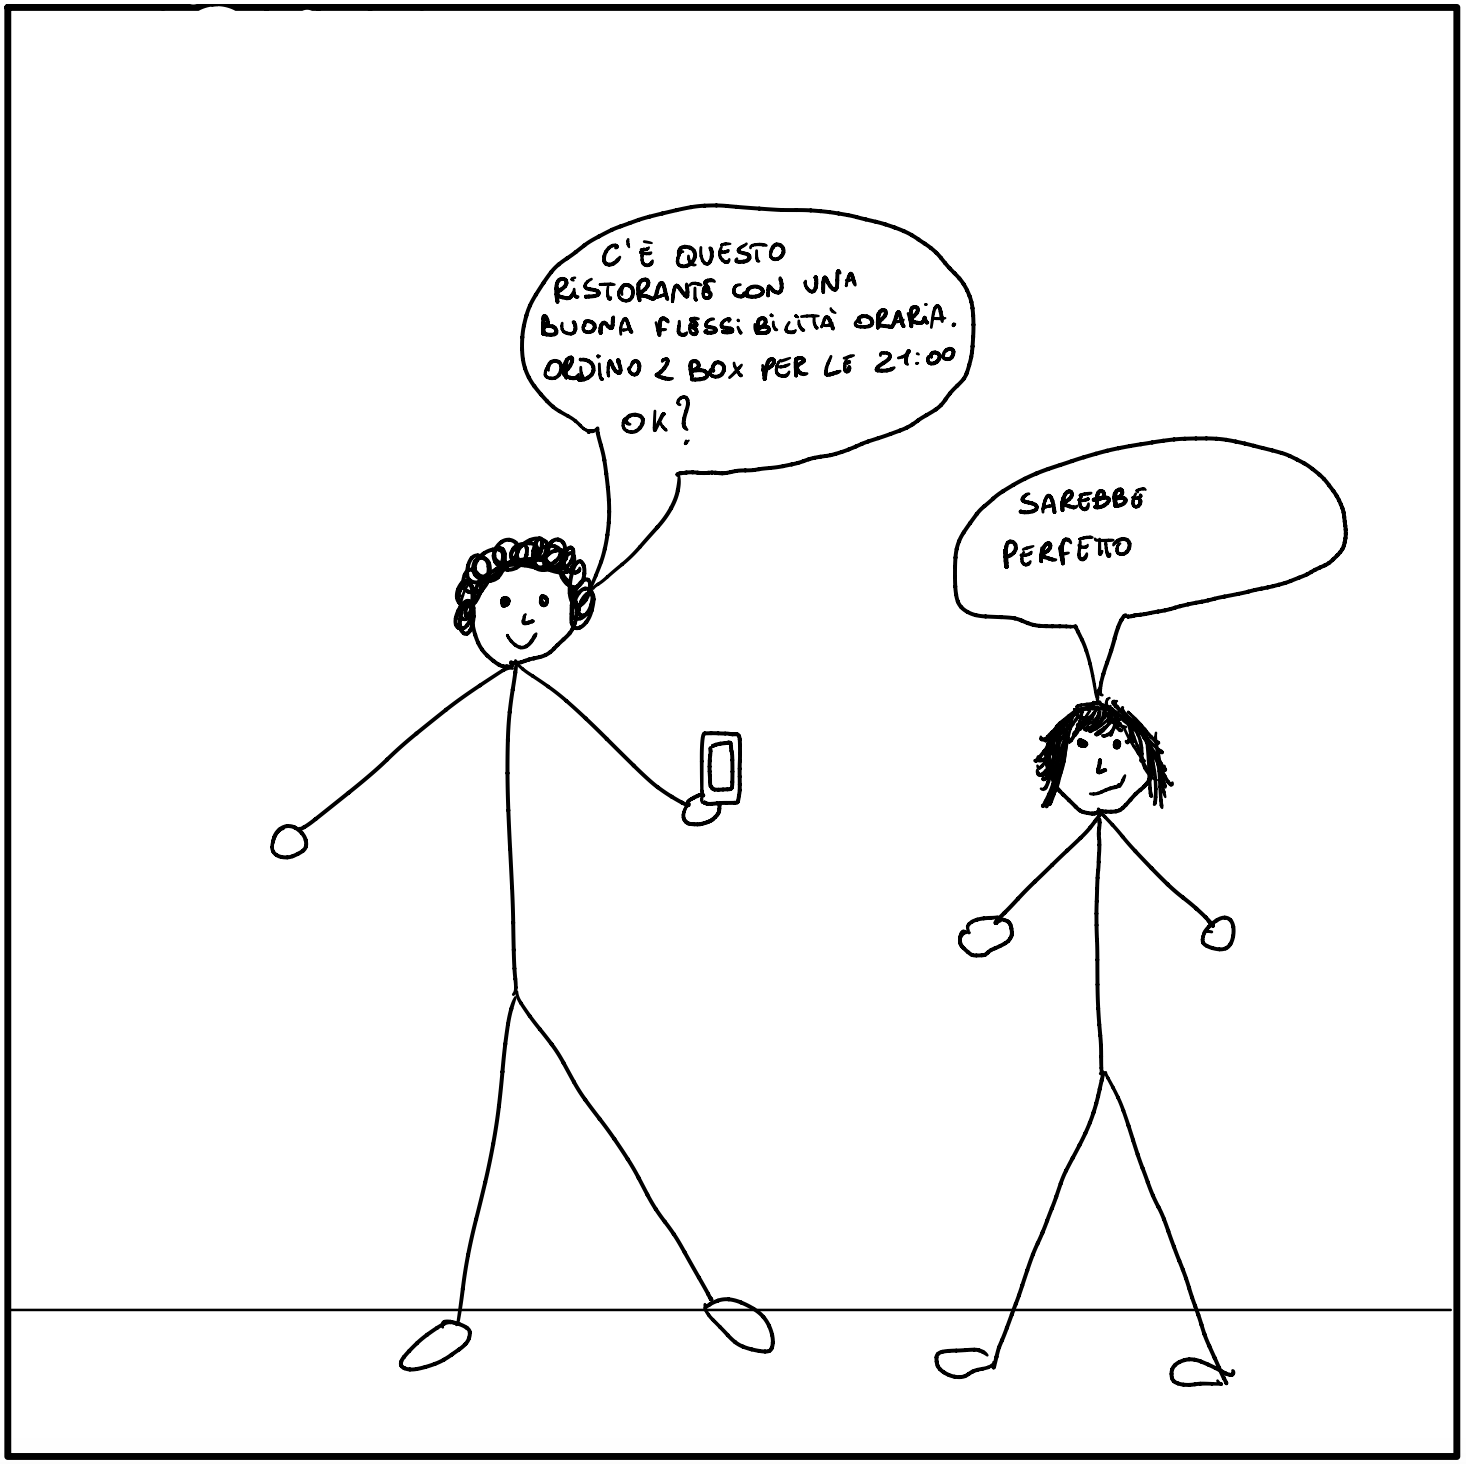
\includegraphics[width=0.3\textwidth]{Storyboard/task3-img/t3.3.png} \\
        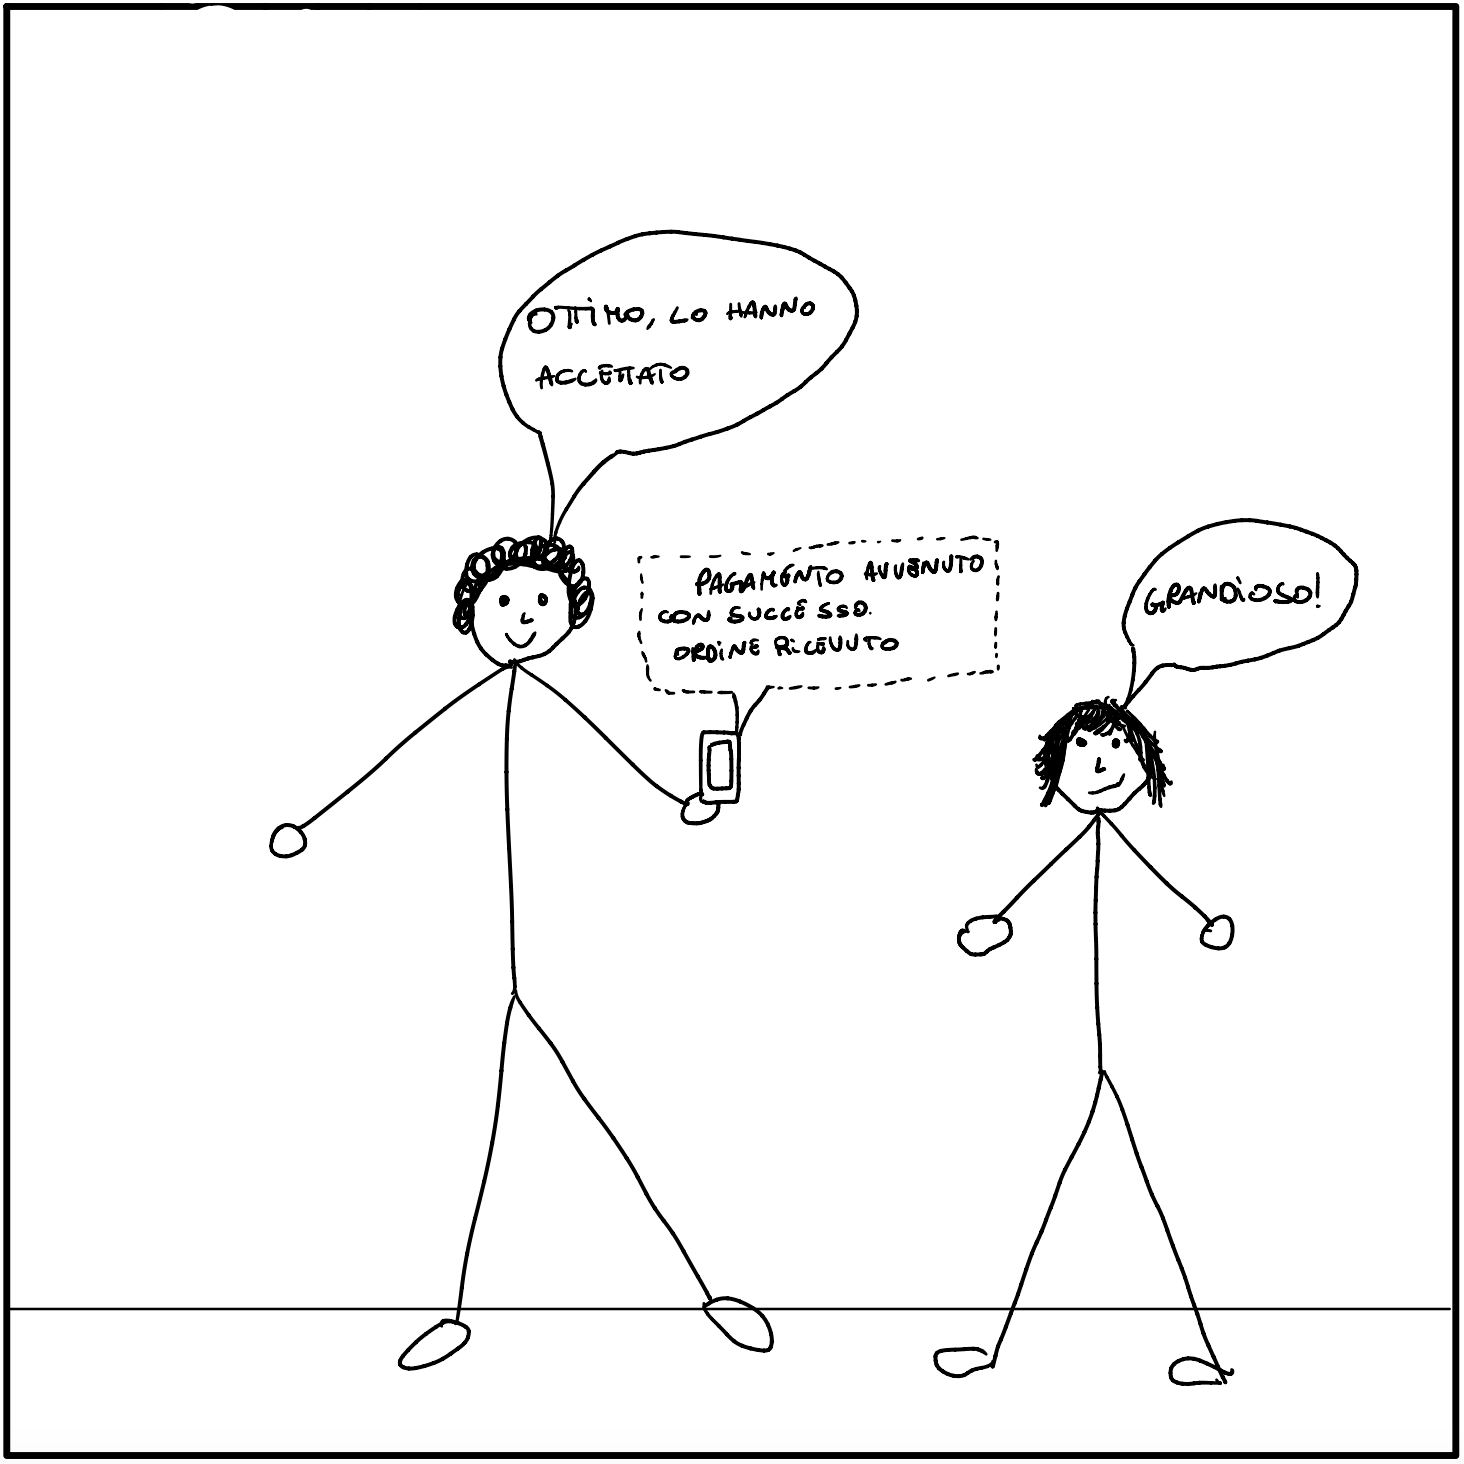
\includegraphics[width=0.3\textwidth]{Storyboard/task3-img/t3.4.png} & & \\
    \end{tabular}
    \label{fig:task2}
\end{figure}

\section{Prototyping}





\end{document}
